\documentclass[usenames,dvipsnames]{beamer}
\usepackage[dvipsnames]{xcolor}

\usepackage{tikz}
\usetikzlibrary{backgrounds,fit, positioning,shapes}
\usetikzlibrary{overlay-beamer-styles}
\usetikzlibrary{shapes.geometric, arrows,backgrounds,fit,positioning}
\usepackage{mathtools}
\usepackage{url}
\def\UrlBreaks{\do\/\do-}
\usepackage{caption}
\newcommand{\source}[1]{\caption*{\tiny Adapted from: {#1}} }
\newcommand{\eqcolon}{\mathrel{\resizebox{\widthof{$\mathord{=}$}}{\height}{ $\!\!=\!\!\resizebox{1.2\width}{0.8\height}{\raisebox{0.23ex}{$\mathop{:}$}}\!\!$ }}}

\usepackage[absolute,overlay]{textpos}

\usetheme[sectionpage=none, progressbar=frametitle, numbering=fraction]{metropolis}        % Use metropolis theme  
% \title{Title}
% \date{\today}
% \author{Author}
% \institute{Title}

% logo of my university
\titlegraphic{%
  \begin{picture}(0,0)
    \put(190,15){\makebox(0,0)[rt]{
\includegraphics[width=2.5cm]{Images/polimi_name_bn.png}}}
  \end{picture}}
\AtBeginSection[]{
\begin{frame}{Talk Overview}
\tableofcontents[currentsection]
\end{frame}
\frame{\sectionpage}
}

\mode<presentation>
{
	\usetheme{metropolis}  
	%\usetheme{boxes}      % or try Darmstadt, Madrid, Warsaw, ...
	%\usecolortheme{crane} % or try albatross, beaver, crane, ...
	\usecolortheme{default}
	\usefonttheme{default}  % or try serif, structurebold, ...
	\useinnertheme{circles}
	\setbeamertemplate{navigation symbols}{}
	\setbeamertemplate{caption}[numbered]
} 

\addtobeamertemplate{navigation symbols}{}{%
	\usebeamerfont{footline}%
	\usebeamercolor[fg]{footline}%
	\hspace{1em}%
	%\insertframenumber/\inserttotalframenumber
}

\newcommand{\backupbegin}{
	\newcounter{framenumberappendix}
	\setcounter{framenumberappendix}{\value{framenumber}}
}
\newcommand{\backupend}{
	\addtocounter{framenumberappendix}{-\value{framenumber}}
	\addtocounter{framenumber}{\value{framenumberappendix}} 
}

% \newsavebox{\authbox}
% \sbox{\authbox}{%
% 	\centering
% 	\begin{minipage}{0.45\linewidth}
% 		\centering\normalsize
% 		\textit{Author}: \par
% 		Alessandro Miola
% 	\end{minipage}
% 	\hfill
% 	\begin{minipage}{0.45\linewidth}
% 		\centering\normalsize
% 		\textit{Supervisors}: \par
% 		Daniele Marazzina \\
% 		Ferdinando M. Ametrano
% 	\end{minipage}
% }

% \bigskip
% \title{Addressing Privacy and Fungibility Issues in Bitcoin: Confidential Transactions}
% \subtitle{}
% \author[Alessandro Miola]{%
% 	\usebox{\authbox}
% }

% \bigskip

% \institute{School of Industrial and Information Engineering \\
% 	Master of Science in Mathematical Engineering}
% \date{20$^{\text{th}}$ December 2018}
% \titlegraphic{%
% 	\begin{picture}(0,0)
% 	\put(30, 230){\makebox(0,0)[rt]{
\includegraphics[width=2cm]{Images/polimi_name_bn.png}}}
% 	\end{picture}}

\title{Addressing Privacy and Fungibility Issues in Bitcoin: Confidential Transactions}
\date{20$^{\text{th}}$ December 2018}
\author{\textbf{Alessandro Miola} \qquad \qquad \qquad 
Supervisors: Daniele Marazzina,\\ \hspace*{6.78cm} Ferdinando M. Ametrano}
%\institute{Politecnico di Milano}

\setbeamertemplate{bibliography entry title}{}
\setbeamertemplate{bibliography entry location}{}

\begin{document}
	\AtBeginSection[]{
	\begin{frame}[noframenumbering]{Outline}
		\small \tableofcontents[currentsection, hideothersubsections]
	\end{frame} 
	}

    \begin{frame}
        \maketitle
    \end{frame}
    
    \begin{frame}{Introduction}
        \begin{itemize}
            \item Privacy is fundamental in every financial and monetary system. Bitcoin should not make any exception.
            \item Bitcoin is neither confidential nor anonymous, but rather pseudonymous.
            \item Both Bitcoin's blockchain structure and security model seem not to be ideal for privacy.
            \item Lack of privacy even affects Bitcoin's capacity to serve as money $\Rightarrow$ detrimental for fungibility: not all bitcoins are equal.
        \end{itemize}
    \end{frame}
    
    \section{Transactions in Bitcoin}
    \begin{frame}{Bitcoin's transactions}
        \begin{itemize}
            \item bitcoins exist as \textit{unspent transaction outputs} (UTXO).
            \item Transaction \color{red}outputs \color{black}are indivisible chunks of currency recorded on the blockchain and associated to addresses:
            \begin{itemize}
                \item they embed the amount and the mathematical puzzle (\textit{locking script}) which determines the conditions for spending.
            \end{itemize}
            \item List of \color{blue}inputs \color{black} referencing and spending UTXO and generating new ones:
            \begin{itemize}
                \item they holds a pointer to the consumed UTXO and the \textit{unlocking script} satisfying the conditions for spending;
                \item the unlocking script generally must hold a digital signature proving ownership of the referenced output.
            \end{itemize}
        \end{itemize}
    \end{frame}
    
    % \begin{frame}{}
    % \tikzset{
    % block/.style={draw, rectangle, rounded corners,
    %     text width=2.2em, text centered, minimum height=3em, minimum width=3.0cm},
    % line/.style={draw, -latex'},
    % int/.style={draw, rectangle, rounded corners, minimum            size=2em, text centered, minimum width=2.5cm},
    % double/.style={draw, rounded corners, rectangle                  split,rectangle split parts=2},
    % triple/.style={draw, rounded corners, rectangle                  split,rectangle split parts=3},
    % quadruple/.style={draw, rounded corners, rectangle               split,rectangle split parts=4},
    % quintuple/.style={draw, rounded corners, rectangle               split,rectangle split parts=5}}
    
    % \begin{tikzpicture}
    % \begin{center}
    % % Place nodes
    
    % \onslide<2->{
    % \node[int, triple] (i1) at (-0.25in, 0in) {\color{blue}TxOut 1.1
    % \nodepart{second} \color{blue}TxOut 1.2
    % \nodepart{third} \color{red}TxOut 1.4};
    % \node[int, below=2mm of i1, triple] (i2) {\color{blue}TxOut 1.3
    % \nodepart{second} \color{red}TxOut 1.5
    % \nodepart{third} \color{red}TxOut 1.6};
    % \node[fit= (i1) (i2), label=above:{Block 1}, draw, minimum width=2.0cm] (Block1) {};
    % % Draw edges
    % \path [line] (i1.one west) -- node[swap,sloped] +(210:0.75);
    % \path [line] (i1.two west) -- node[swap,sloped] +(210:0.75);
    % \path [line] (i2.one west) -- node[swap,sloped] +(210:0.75);
    % }
    % \end{center}
    % \begin{center}
    % \onslide<3->{
    % \node[int, quadruple] (a1) at (1.125in, 0in) {\color{blue}TxOut 1.4
    % \nodepart{second}\color{blue}TxOut 1.5
    % \nodepart{third}\color{red}TxOut 2.1
    % \nodepart{fourth}\color{red}TxOut 2.2};
    % \node[int, below=2mm of a1, triple] (a2) {\color{blue}TxOut 1.6
    % \nodepart{second}\color{red}TxOut 2.3
    % \nodepart{third}\color{red}TxOut 2.4};
    % \node[fit= (a1) (a2),label=above:{Block 2}, draw, minimum width=2.0cm] (Block2) {};
    % % Draw edges
    % \path [line] (a1.one west) -- (i1.three east);
    % \path [line] (a1.two west) -- (i2.two east);
    % \path [line] (a2.one west) -- (i2.three east);
    % }
    % \end{center}
    
    % \begin{center}
    % \onslide<4->{
    % \node[int, quadruple] (b1) at (2.5in, 0in) {\color{blue}TxOut 2.1
    % \nodepart{second}\color{blue}TxOut 2.2
    % \nodepart{third}\color{red}TxOut 3.1
    % \nodepart{fourth}\color{red}TxOut 3.2};
    % \node[int, below=2mm of b1, triple] (b2) {\color{blue}TxOut 2.3
    % \nodepart{second}\color{blue}TxOut 2.4
    % \nodepart{third}\color{red}TxOut 3.3};
    % \node[fit= (b1) (b2), label=above:{Block 3}, draw, minimum width=2.0cm] (Block3) {};
    % \path [line] (b1.one west) -- (a1.three east);
    % \path [line] (b1.two west) -- (a1.four east);
    % \path [line] (b2.one west) -- (a2.two east);
    % \path [line] (b2.two west) -- (a2.three east);
    % }
    % \end{center}
    % \end{tikzpicture}
    % \vfill
    % \vfill
    % \begin{center}
    % \begin{tikzpicture}
    % \onslide<1>{
    % \node[int, quadruple, label=above:{UTXO set}] (UTXO) {TxOut 1.1
    % \nodepart{second} TxOut 1.2
    % \nodepart{third} TxOut 1.3};
    % }{\onslide<2>{\node[int, quadruple, label=above:{UTXO set}] (UTXO) {TxOut 1.4
    % \nodepart{second} TxOut 1.5
    % \nodepart{third} TxOut 1.6};
    % }}{\onslide<3>{\node[int, quadruple, label=above:{UTXO set}] (UTXO) {TxOut 2.1
    % \nodepart{second} TxOut 2.2
    % \nodepart{third} TxOut 2.3
    % \nodepart{fourth} TxOut 2.4};
    % }}
    % {\onslide<4>{\node[int, quadruple, label=above:{UTXO set}] (UTXO) {TxOut 3.1
    % \nodepart{second} TxOut 3.2
    % \nodepart{third} TxOut 3.3};
    % }};
    % \end{tikzpicture}
    % \end{center}
    % \end{frame}
    
    % \begin{frame}{Scripting language}
        
    % \end{frame}
        
    \section{Privacy and Fungibility issues}
        \begin{frame}{Privacy}
            \begin{itemize}
                \item Transactional graph privacy: who is paying who?
                \begin{itemize}
                    \item Linkability of transactions;
                    \item bad users' practices (\textit{address reuse}).
                \end{itemize}
                \item Value privacy: how much is one paying or receiving?
                \begin{itemize}
                    \item Unencrypted transaction amounts.
                \end{itemize}
                \item Identity privacy: who is behind the coins?
                \begin{itemize}
                    \item Leakage of personal information when accessing exchanges or on-line stores. 
                \end{itemize}
                \item Trade-off: blockchain's transparency $\Leftrightarrow$ Bitcoin's privacy.
            \end{itemize}
        \end{frame}
        
        \begin{frame}{Fungibility}
            \begin{itemize}
                \item Property of a unit of a good to be indistinguishable from any other unit of the same good.
                \item Fundamental property for moneys and currencies:
                \begin{itemize}
                    \item do not want to care of the possibility of possession of banknotes being revoked for their ``bad" history;
                    \item possibility of \textit{blacklisting} banknotes would destroy confidence in receiving them.
                \end{itemize}
                \item Bitcoin is substantially \textit{immediate} and \textit{final} payment; this makes discussion intertwine with money in its cash-like forms.
                \item Trade-off: blockchain's transparency $\Leftrightarrow$ bitcoin's fungibility.
            \end{itemize}
        \end{frame}
    \section{Cryptographic primitives}
    \subsection{Pedersen commitment}
    
    \begin{frame}{Pedersen commitment }
        \begin{itemize}[<+->]
            \item<1-> \textit{Commitment scheme}: keep a piece of data secret, but commit to it to prevent tampering.
            \end{itemize}
            % \only<1>{\begin{block}{Definition.}
            % Let ($\mathbb{G,\circ}$) be an elliptic curve group of prime order $n$. Let $G$, $H$ be fixed \textit{nothing-up-my-sleeves} (NUMS) generator points of $\mathbb{G}$.\\ \ \\
            % The elliptic curve NUMS points are points whose elliptic curve discrete logarithm relative to each other are unknown:
            % \begin{itemize}
            %     \item unknown $x$ s.t. $xG = H$;
            %     \item unknown $y$ s.t. $yH = G$.
            % \end{itemize}
            % \end{block}
            % }
            {\only<1>{\begin{block}{Definition.}
            Let ($\mathbb{G,\circ}$) be an elliptic curve group of prime order $n$. Let $G$, $H$ be two NUMS generators of $\mathbb{G}$; let $r$, $v$ $\in \mathbb{Z}_n$ ($r$ chosen at random). Define a Pedersen commitment $C$ to $v$ by the following scheme:
            \begin{align*}
            commit \colon \mathbb{Z}_n^2 &\to \mathbb{G}\\
            (r,v) &\mapsto rG + vH\\
            open \colon \mathbb{Z}_n^2 \times \mathbb{G} &\to \{True, False\}
            \end{align*}
            such that $open(r, v, C) \mapsto True$ $\forall(r,v)$ in the domain of $commit$.
            \end{block}}}
        \end{frame}
        
        \begin{frame}{Pedersen commitment: properties}
        \begin{itemize}
        \item<1-> \textit{Perfectly hiding} and \textit{computationally binding} commitment scheme.
        \item<2-> \textit{Additively homomorphic} commitment scheme.
        \end{itemize}
        \begin{block}{Definition.}
        % \only<1>{Let ($\mathbb{G,\circ}$) be an elliptic curve group of prime order $n$. Let $C$ denote a (public) commitment. Let $r$, $v$ $\in \mathbb{Z}_n$.\\
        % A commitment scheme is a pair of algorithms: \begin{itemize}
        %     \item $commit(r,v) \rightarrow \mathbb{G}$
        %     \item $open(r,v,C) \rightarrow \{True, False\}$
        % \end{itemize}
        % such that $open(r, v, commit(r,v)) \mapsto True$ $\forall(r,v)$ in the domain of $commit$.}
        \only<1>{A commitment scheme is said to be:
        \begin{itemize}
            \item perfectly (computationally) \textit{hiding} if the distribution of $commit(r,v)$ for uniformly random $r$ is equal (computationally indistinguishable) for fixed values of $v$;
            \item perfectly \textit{binding} if $\forall(r,v)$ in the domain of $commit$, $\nexists(r',v') \neq (r,v)$: $open(r',v',commit(r,v)) \mapsto True$; computationally \textit{binding} if no PPT (probabilistic polynomial time) algorithm can produce such $(r',v')$ with non-negligible probability.
        \end{itemize}}
    

        {\only<2>{%\begin{block}{Definition.}
        A commitment scheme is \textit{additively homomorphic} if:\begin{itemize}
            \item $commit(r,v) + commit(r',v') = commit(r+r', v+v')$.
            %\item $commit(r,v) + commit(r',v')$ {$\buildrel d \over \sim$} $commit(r+r', v+v')$.
            \end{itemize}}}
        \end{block}
        \end{frame}
    
    \subsection{Zero-Knowledge proofs of knowledge}
    \begin{frame}{Zero-Knowledge proof of knowledge}
        \begin{itemize}[<+->]
            \item<1-> Proof that yields nothing but its validity.
            \begin{itemize}
                \item<1-> Alice tries to convince Bob of being in possession of some secret information.
                \item<1-> Proof performed in Zero-Knowledge.
            \end{itemize}
        \end{itemize}
        % \begin{columns}
        % \begin{column}{0.55\linewidth}
        \begin{figure}
            \centering
            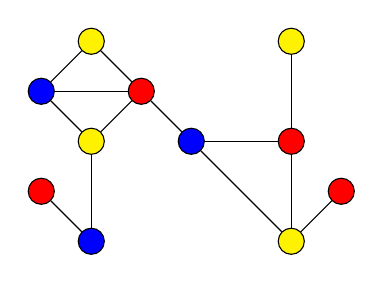
\begin{tikzpicture}[-]%,>=stealth',shorten >=1pt]
            \node[draw, circle, fill=yellow] (e0) at (-0.5in, 0.5in){};
            \node[draw, circle, fill=blue] (e1) at (-0.75in, 0.25in){};
            \node[draw, circle, fill=red] (e2) at (-0.25in, 0.25in){};
            \node[draw, circle, fill=yellow] (e3) at (-0.5in, 0in){};
            \node[draw, circle, fill=blue] (e4) at (0in, 0in){};
            \node[draw, circle, fill=blue] (e5) at (-0.5in, -0.5in){};
            \node[draw, circle, fill=red] (e6) at (-0.75in, -0.25in){};
            \node[draw, circle, fill=yellow] (e7) at (0.5in, -0.5in){};
            \node[draw, circle, fill=yellow] (e8) at (0.5in, 0.5in){};
            \node[draw, circle, fill=red] (e9) at (0.5in, 0in){};
            \node[draw, circle, fill=red] (e10) at (0.75in, -0.25in){};
            
            \path
            (e0) edge (e1)
            (e1) edge (e2)
            (e2) edge (e3)
            (e3) edge (e1)
            (e2) edge (e0)
            (e3) edge (e5)
            (e5) edge (e6)
            (e2) edge (e4)
            (e4) edge (e9)
            (e4) edge (e7)
            (e7) edge (e9)
            (e7) edge (e10)
            (e8) edge (e9);
            
            \end{tikzpicture}
            \caption{Graph 3-colorability problem}
        \end{figure}
    \end{frame}
    
    \subsection{Ring signatures}
    \begin{frame}{Ring signature}
        \begin{itemize}%[<+->]
            % \item<1-> \textit{Signer-ambiguous} digital signature scheme allowing for any actor in a group to sign on behalf of the group.
            % \begin{itemize}
            %     \item Multiparty $1$-of-$r$ signature scheme without cooperation from the other $r-1$ members.
            % \end{itemize}
            \item OR proof: given a ring of $r$ public keys \{$\color{ForestGreen}Q_0\color{black}, \dots, \color{ForestGreen}Q_{r-1}$\color{black}\}, the ambiguous signer proves to know \{$\color{red}q_0$ \color{black}OR $\color{red}q_1$ \color{black}OR $\dots$ \color{black}OR $\color{red}q_{r-1}$\color{black}\}.
        \end{itemize}
        \begin{figure}
            \centering
            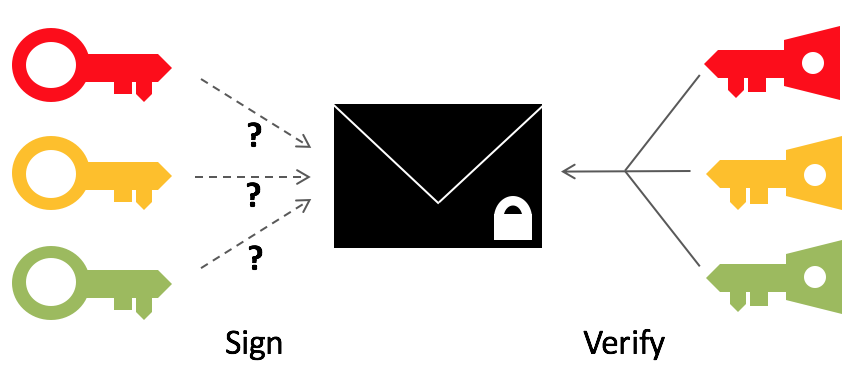
\includegraphics[scale = 0.5]{Images/Ring.png}
            \caption{Ring signature scheme}
        \end{figure}
        \begin{itemize}
            % \alt<3>{\\ \ \\\textit{Sign}:
            % \begin{itemize}
            %     \item Pick up a random nonce $k$ $\rightarrow$ $K = kG$;
            %     \item given the message $m$ to be signed, compute $hash(K||m)$ $\rightarrow$ $e = hash(K||m)$;
            %     \item sign as follows: $s = k + eq$;
            %     \item publish ($s, e, m$).
            % \end{itemize}}{
            % \only<4>{\\ \ \\\textit{Verify}. Given \{$s, e, m, Q$\} as inputs:
            % {\begin{itemize}
            %     \item compute $sG - eQ$: $sG - eQ = sG - eqG = (s - eq)G = kG = K$;
            %     \item compute $e' = hash(K||m)$;
            %     \item verify whether $e' = e$; if so, the signature is valid.
            %\end{itemize}}}}
            \item Tool for whistleblowing.
        \end{itemize}
    \end{frame}
    \begin{frame}{Ring signature}
        \alt<1>{\begin{columns}
        \begin{column}{0.635\linewidth}
				\onslide<1> {AOS\_SIGN($m$, $q_{i^{*}}$, $Q_i$: $0 \leq i \leq r-1)$:
				\begin{enumerate}
					\item $k_{i^{*}} \xleftarrow{\text{\$}} \{1,\dots,n-1\}$;
					\item $K_{i^{*}} \gets k_{i^{*}}G$;\\
					\item for $i \gets i^{*}+1, \dots, r-1, 0, \dots, i^{*}-1$
					\begin{enumerate}
					    \item $e_i \gets hash(K_{i-1}||m||i) $;
					    \item $s_i \xleftarrow{\text{\$}} \{1,\dots,n-1\}$;
					    \item $K_i \gets s_iG - e_iQ_i$;
					\end{enumerate}
					\item $e_{i^{*}} \gets hash(K_{i^{*}-1}||m||i^{*}) $;
					\item $s_{i^{*}} \gets k_{i^{*}} + e_{i^{*}}q_{i^{*}}$;
					\item \textbf{return} ($e_0, s_0, \dots, s_{r-1}$)$\eqcolon \sigma$
				\end{enumerate}}
			\end{column}
	\begin{column}{0.365\linewidth}
	\begin{figure}
    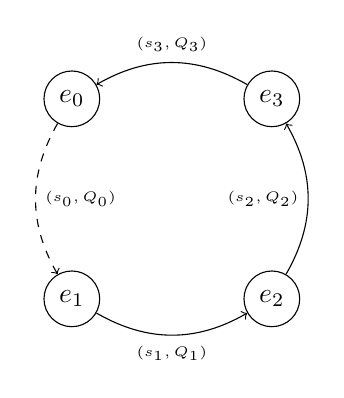
\begin{tikzpicture}[->]%,>=stealth',shorten >=1pt]
    \node[draw, circle] (e0) at (-0.5in, 0.5in)     {$\textcolor{black!100}{e_0}$};
    \node[draw, circle] (e1) at (-0.5in, -0.5in)   {$\textcolor{black!100}{e_1}$};
    \node[draw, circle] (e2) at (0.5in, -0.5in)  {$\textcolor{black!100}{e_2}$};
    \node[draw, circle] (e3) at (0.5in, 0.5in)  {$\textcolor{black!100}{e_3}$};

    \path
    (e0) edge[bend right, dashed] node[right] {\tiny{\textcolor{black!100}{$(s_0, Q_0)$}}} (e1)
    (e1) edge[bend right] node[below = 0.5pt] {\tiny{\textcolor{black!100}{$(s_1, Q_1)$}}} (e2)
    (e2) edge[bend right] node[left] {\tiny{\textcolor{black!100}{$(s_2, Q_2)$}}} (e3)
    (e3) edge[bend right] node[above = 0.5pt] {\tiny{\textcolor{black!100}{$(s_3, Q_3)$}}} (e0);
    \end{tikzpicture}
    \only{\caption{AOS ring signature (1-of-4)}{}}
    \only{\source{\cite{Borromean}}}
    \end{figure}
	\end{column}
    \end{columns}}
    %\end{frame}
    
    %\begin{frame}{AOS ring signature}
        {\only<2>{\begin{columns}
        \begin{column}{0.635\linewidth}
				\onslide<2> {AOS\_VERIFY($m$, $\sigma$, $Q_i$: $0 \leq i \leq r-1)$:
				\begin{enumerate}
					\item for $i \gets 0, \dots, r-1$
					\begin{enumerate}
					    \item $K_i \gets s_iG - e_iQ_i$;
					    \item $e_{i+1\%r} \gets hash(K_i||m||i+1\%r)$;
					\end{enumerate}
					\item \textbf{if} $e_0 = 0$ or $e_0 \geq n$: \\ \textbf{\ \ \ return} False;\\
					\item \textbf{if} $e_0 = \sigma[0]$:
					\\ \textbf{\ \ \ return} True;\\
				\end{enumerate}}
			\end{column}
	\begin{column}{0.365\linewidth}
	\begin{figure}
    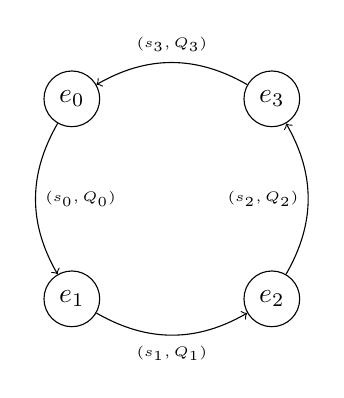
\begin{tikzpicture}[->]%,>=stealth',shorten >=1pt]
    \node[draw, circle] (e0) at (-0.5in, 0.5in)     {$\textcolor{black!100}{e_0}$};
    \node[draw, circle] (e1) at (-0.5in, -0.5in)   {$\textcolor{black!100}{e_1}$};
    \node[draw, circle] (e2) at (0.5in, -0.5in)  {$\textcolor{black!100}{e_2}$};
    \node[draw, circle] (e3) at (0.5in, 0.5in)  {$\textcolor{black!100}{e_3}$};

    \path
    (e0) edge[bend right] node[right] {\tiny{\textcolor{black!100}{$(s_0, Q_0)$}}} (e1)
    (e1) edge[bend right] node[below = 0.5pt] {\tiny{\textcolor{black!100}{$(s_1, Q_1)$}}} (e2)
    (e2) edge[bend right] node[left] {\tiny{\textcolor{black!100}{$(s_2, Q_2)$}}} (e3)
    (e3) edge[bend right] node[above = 0.5pt] {\tiny{\textcolor{black!100}{$(s_3, Q_3)$}}} (e0);
    \end{tikzpicture}
    \only{\caption{AOS ring signature verification (1-of-4)}}
    \only{\source{\cite{Borromean}}}
    \end{figure}
	\end{column}
    \end{columns}}}
    \end{frame}
    
    % \subsection{Elliptic curve Diffie-Hellman}
    % \begin{frame}{ECDH Key Exchange protocol}
    % \begin{itemize}
    %     \item Key agreement scheme based on elliptic curve cryptography.
    %     \item Establish a shared secret between two parties over an insecure (yet authenticated) channel.
    % \end{itemize}
    % \begin{center}
    %     \begin{figure}
    %         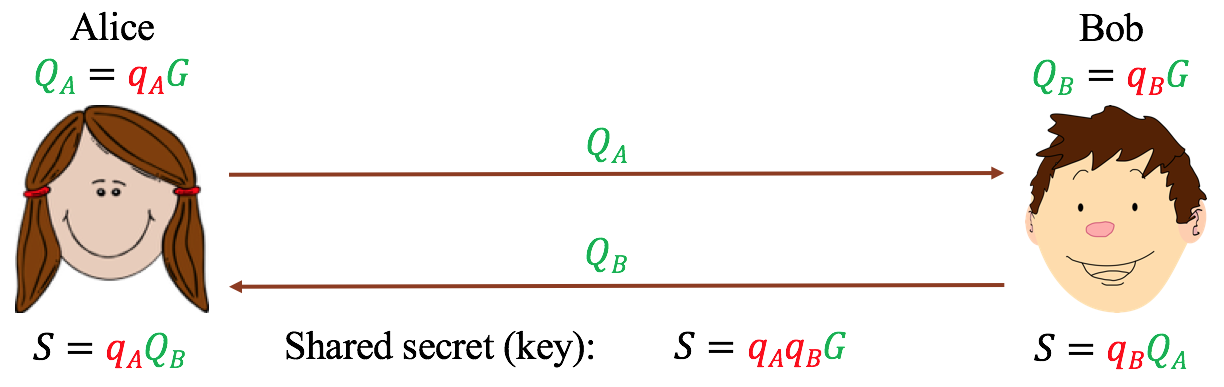
\includegraphics[scale = 0.5]{Images/ECDH.png}
    %         \captionof{figure}{ECDH key exchange}
    %     \end{figure}
    % \end{center}
    % \begin{itemize}
    %     \item Channel authentication required to prevent \textit{man-in-the-middle} attacks.
    % \end{itemize}
    % \end{frame}
    
    \section{Confidential Transactions}
    
    \subsection{Overview}
    \begin{frame}{Confidential Transactions}
        \begin{itemize}
            \item Proposal for a transactional format with encrypted amounts, which requires the same  cryptographic assumptions of Bitcoin (hardness of ECDLP).
            \item Built through homomorphic encryption without compromising the possibility for the nodes to verify the validity of each transaction.
            \item It provides \textit{value privacy}.
        \end{itemize}
    \end{frame}
    
    \subsection{Output amount encryption \& consequences}
    \begin{frame}{Pedersen commitment in CT}
        \begin{itemize}
            \item Substitute 8-byte output amounts in the clear with \textit{perfectly hiding} 33-byte Pedersen commitments to the amounts.
            \item Interpretation of the parameters:
            \begin{itemize}
                \item $r$: secret random \textit{blinding factor};
                \item $v$: committed \textit{output amount}.
            \end{itemize}
        \end{itemize}\\
        \begin{equation*}
            \color{ForestGreen}v_{i1} \color{black}= \color{ForestGreen}v_{o1} \color{black}+ \color{ForestGreen}v_{o2} \color{black}+ \color{ForestGreen}fee
        \end{equation*} 
        $\qquad \qquad \qquad \qquad \qquad \qquad \qquad \Downarrow$
        \begin{equation*}
            (\color{red}r_{i1}\color{ForestGreen}G \color{black}+ \color{red}v_{i1}\color{ForestGreen}H \color{black}) = (\color{red}r_{o1}\color{ForestGreen}G \color{black}+ \color{red}v_{o1}\color{ForestGreen}H \color{black}) + (\color{red}r_{o2}\color{ForestGreen}G \color{black}+ \color{red}v_{o2}\color{ForestGreen}H \color{black})+ \color{ForestGreen}fH
        \end{equation*}
        $\qquad \qquad \qquad \qquad \qquad \qquad \qquad \Downarrow$
        \begin{equation*}
            r_{i1} = r_{o1} + r_{o2}
        \end{equation*}
        \begin{equation*}
            v_{i1} = v_{o1} + v_{o2} + f
        \end{equation*}
    \end{frame}
    
    % \begin{frame}{Setting of the blinding factors}
    %     \begin{minipage}{.25\textwidth}
    %     \centering
    %     
\includegraphics[,     width=.75\textwidth]{Images/Alice.png}
    %     \end{minipage}%
    %     \begin{minipage}{.75\textwidth}
    %     \begin{itemize}
    %     \item \textit{Blinding factor} from input is already set; \quad $\rightarrow$ \quad $r_{o1} = r_{i1} - r_{o2}$.
    %     \end{itemize}
    %     \end{minipage}
        
    %     \begin{minipage}{.75\textwidth}
    %     \begin{itemize}
    %     \item He gets ownership of the first output with knowledge of amount and blinding factor $r_{o1}$ (no disclosure of $r_{i1}$ and $r_{o2}$).
    %     \end{itemize}
    %     \end{minipage}%
    %      \begin{minipage}{.25\textwidth}
    %     \centering
    %     
\includegraphics[,     width=.75\textwidth]{Images/Bob.png}
    %     \end{minipage}%
        
    %     \begin{minipage}{.25\textwidth}
    %     \centering
    %     
\includegraphics[,     width=.75\textwidth]{Images/Carl.png}
    %     \end{minipage}%
    %     \begin{minipage}{.75\textwidth}
    %     \begin{itemize}
    %     \item He verifies transaction validity.
    %     \end{itemize}
    %     \end{minipage}%
    % \end{frame}
    
    \begin{frame}{Commitment to value 0}
        \begin{itemize}
            \item Instrumental in verifying the validity of each transaction.
            \item A commitment $C = rG$ gives the opportunity to produce a digital signature with the commitment as public key:
            \begin{itemize}
                \item by definition, a signature with private key \color{red} $q$ \color{black} can be verified with public key $\color{red}q\color{ForestGreen}G$\color{black};
                \item if $v\neq0$, it is infeasible to find \color{red} $q$ \color{black}such that $\color{red}q\color{ForestGreen}G \color{black}= \color{red}r\color{ForestGreen}G \color{black}+ \color{red}v\color{ForestGreen}H$.
            \end{itemize}
        \end{itemize}
        $\qquad \qquad \qquad \qquad \qquad \qquad \qquad \Downarrow$
        \begin{center}
        A Pedersen commitment can be proven to be a commitment to $v=0$ by signing the transaction with $\color{red}r$ \color{black}as private key, $\color{ForestGreen}C$ \color{black}as public key.
        \end{center}
    \end{frame}
    
    \subsection{Zero-Knowledge range proofs}
    \begin{frame}{Zero-Knowledge range proof}
        \underline{Reason for}:
        \begin{itemize}
            \item addition is modular and wraps around;
            \item possible to create money from nothing.
        \end{itemize}
    \begin{block}{Example.}
    Consider a curve built on a finite field of prime order $n=13$.\\ \ \\
    \end{block}
    \begin{columns}
    \begin{column}{0.5\linewidth}
    \makebox[\textwidth]{
    \begin{tabular}{|c|c|}
			\hline
			Inputs & Outputs \\
			\hline
			$C(r_{i1},2)$ & $C(r_{o1},8)$ \\
			 & $C(r_{o2},7)$ \\
			\hline
	\end{tabular}
	}\captionof{table}{Example of wrapping}
    \end{column}
    \begin{column}{0.5\linewidth}
    \makebox[\textwidth]{
    \begin{tabular}{|c|c|}
			\hline
			Inputs & Outputs \\
			\hline
			$C(r_{i1},2)$ & $C(r_{o1},5)$ \\
			 & $C(r_{o2},-3)$ \\
			\hline
	\end{tabular}
	}\captionof{table}{Negative amounts}
    \end{column}
    \end{columns}
    \centering Additional piece of data proving that each committed output is in a given range ensuring that no overflow is possible and the amount is non-negative.
    \end{frame}
    
    \begin{frame}{Enforce Zero-Knowledgeness: Borromean ring signature}
    \begin{itemize}
        \item Given $r$ rings of public keys, the ambiguous signer proves to know one of \{$\color{red}q_{0,0}$ \color{black}OR $\color{red}q_{0,1}$ \color{black}OR $\dots$\} AND one of \{$\color{red}q_{1,0}$ \color{black}OR $\color{red}q_{1,1}$ \color{black}OR $\dots$\} AND $\dots$ AND one of \{$\color{red}q_{{r-1},{0}}$ \color{black}OR $\color{red}q_{{r-1},{1}}$ \color{black}OR $\dots$\}.
    \end{itemize}
    \only<1>{\begin{figure}%\advance\leftskip-0.25cm
    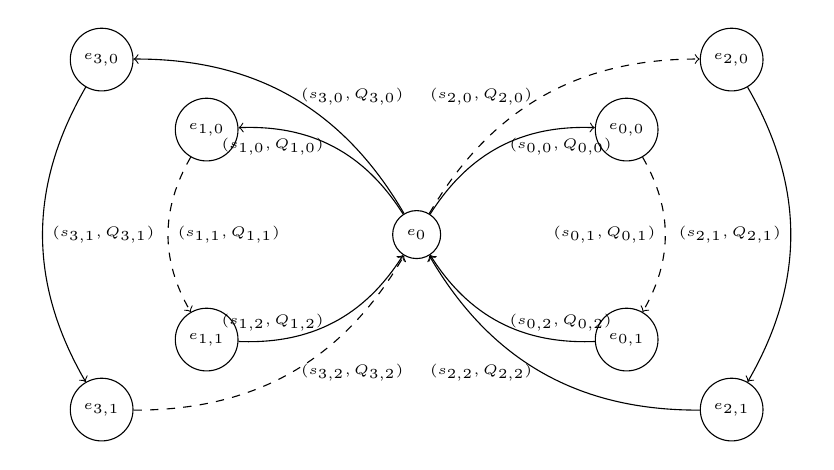
\begin{tikzpicture}[->,scale = 0.7]%,>=stealth',shorten >=1pt]
    \node[draw, circle] (e0) at (0in, 0in)     {\tiny{$\textcolor{black!100}{e_0}$}};
    \node[draw, circle] (e1) at (1.5in, 0.75in)   {\tiny{$\textcolor{black!100}{e_{0,0}}$}};
    \node[draw, circle] (e2) at (1.5in, -0.75in)  {\tiny{$\textcolor{black!100}{e_{0,1}}$}};
    \node[draw, circle] (e3) at (-1.5in, 0.75in)  {\tiny{$\textcolor{black!100}{e_{1,0}}$}};
    \node[draw, circle] (e4) at (-1.5in, -0.75in) {\tiny{$\textcolor{black!100}{e_{1,1}}$}};
    \node[draw, circle] (e1_bis) at (2.25in, 1.25in)     {\tiny{$\textcolor{black!100}{e_{2,0}}$}};
    \node[draw, circle] (e1_ter) at (-2.25in, 1.25in)     {\tiny{$\textcolor{black!100}{e_{3,0}}$}};
    \node[draw, circle] (e2_bis) at (-2.25in, -1.25in)     {\tiny{$\textcolor{black!100}{e_{3,1}}$}};
    \node[draw, circle] (e2_ter) at (2.25in, -1.25in)     {\tiny{$\textcolor{black!100}{e_{2,1}}$}};

    % left circle
    \path
    (e0) edge[bend right] node[left] {\tiny{\textcolor{black!100}{$(s_{1,0}, Q_{1,0})$}}} (e3)
    (e3) edge[bend right, dashed] node[right] {\tiny{\textcolor{black!100}{$(s_{1,1}, Q_{1,1})$}}} (e4)
    (e4) edge[bend right] node[left] {\tiny{\textcolor{black!100}{$(s_{1,2}, Q_{1,2})$}}} (e0)
    (e0) edge[bend right] node[right] {\tiny{\textcolor{black!100}{$(s_{3,0}, Q_{3,0})$}}} (e1_ter)
    (e1_ter) edge[bend right] node[right] {\tiny{\textcolor{black!100}{$(s_{3,1}, Q_{3,1})$}}} (e2_bis)
    (e2_bis) edge[bend right, dashed] node[right] {\tiny{\textcolor{black!100}{$(s_{3,2}, Q_{3,2})$}}} (e0);
  % right circle
  \path
    (e0) edge[bend left] node[right] {\tiny{\textcolor{black!100}{$(s_{0,0}, Q_{0,0})$}}} (e1)
    (e1) edge[bend left, dashed] node[left] {\tiny{\textcolor{black!100}{$(s_{0,1}, Q_{0,1})$}}} (e2)
    (e2) edge[bend left] node[right] {\tiny{\textcolor{black!100}{$(s_{0,2}, Q_{0,2})$}}} (e0)
    (e0) edge[bend left, dashed] node[left] {\tiny{\textcolor{black!100}{$(s_{2,0}, Q_{2,0})$}}} (e1_bis)
    (e1_bis) edge[bend left] node[left] {\tiny{\textcolor{black!100}{$(s_{2,1}, Q_{2,1})$}}} (e2_ter)
    (e2_ter) edge[bend left] node[left] {\tiny{\textcolor{black!100}{$(s_{2,2}, Q_{2,2})$}}} (e0);
    \end{tikzpicture}
    \captionof{figure}{Borromean ring signatures}
    \label{fig:Borromean_ringg}
    \end{figure}}
    \only<2> {
        \\ \ \\
        \\ \ \\
        \makebox[\textwidth]{
		\begin{tabular}{|c|c|}
			\hline
			& Signature size \\
			\hline
			$r$ AOS ring signatures & $r\cdot N + r$ (32-bytes numbers) \\
			\hline
			Borromean ring signature & $r\cdot N + 1$ (32-bytes numbers) \\
			\hline
			$\Delta$ & $\textbf{r - 1}$ (32-bytes numbers) \\
			\hline
		\end{tabular}
	}\captionof{table}{Borromean ring signature: signature size}}
    \end{frame}
    
    \begin{frame}{Use of Borromean ring signatures}
        %\underline{Role}: prove that each committed value is in range.\\ \ \\
        \begin{itemize}
            \item Consider the output amount in its base-4 expansion: \begin{center}
            $ v = v_0\cdot 4^0 + v_1\cdot 4^1 + v_2\cdot 4^2 + \dots + v_{15}\cdot 4^{15}$;
            \end{center}
        \end{itemize}
        \textit{Ring-sign} over each digit:
        \begin{itemize}
            \item $C_i = r_iG + v_i4^iH$, $i=0,\hdots,15$;
            \item arrange a ring of signatures per digit with a verification public key per digit value $v_i$, $i=0,\dots,3$;
            \item provide a Borromean ring signature over the rings: \begin{center}
            $\{r_iG + v_i4^iH, r_iG + v_i4^iH - 4^iH, r_iG + v_i4^iH - 2\cdot4^iH, r_iG + v_i4^iH - 3\cdot4^iH\}$
            \end{center}
            % \begin{itemize}
            %     \item the whole commitment ranges in [1,$\sum_{i=0}^{15}v_i\cdot4^i$] satoshi;
            % \end{itemize}
            \item $RP_v = (C_0,\dots,C_{15},\underbrace{e_0,s_{0,0},\dots,s_{0,3},\dots,s_{15,0},\dots,s_{15,3}}_{signature}) $.
        \end{itemize}
    \end{frame}
    
    %\subsection{Transaction data transmission}
    % \begin{frame}{Sender-receiver interaction}
    %     \begin{itemize}
    %         \item Encryption even prevents the receiver to know amount and blinding factor associated to each output.
    %     \end{itemize}
    %     Transmission of:
    %     \begin{itemize}
    %         \item amounts;
    %         \item blinding factors;
    %         \item user-selected data.
    %     \end{itemize}\\ \ \\
    %     \centering$\Rightarrow$ The transfer can happen non-interactively by running an instance of ECDH and exploiting the shared key to deduce the quantities involved.
    % \end{frame}
    
    \section{Conclusions}
    \begin{frame}{Conclusions}\label{lastframe}
        \begin{itemize}
            \item Confidential transactions would provide consistent value privacy in the protocol.
            \item Not ready yet for integration in the Bitcoin protocol as they suffer from excessively burdening each transaction size. 
        \end{itemize}
        However,
        \begin{itemize}
            \item a new and more efficient solution to range proof construction has been proposed, \textit{Bulletproofs}:
            \begin{itemize}
                \item aggregation of range proofs;
                \item batched verification of multiple proofs.
            \end{itemize}
            \item \textit{Mimblewimble}: promising cryptosystem built on confidential transactions.
        \end{itemize}
    \end{frame}
    
%     \begin{frame}
% 		\centering
% 		\huge Thank you for the attention!
% 		\par
% 	\end{frame}
	
    \appendix
    \backupbegin
    \begin{frame}[t, allowframebreaks]
	\frametitle{References}
    	\setbeamertemplate{bibliography item}[text]
    	\bibliographystyle{plain}
		\nocite{*}
		\bibliography{biblio}
	\end{frame}
	
% 	\begin{frame}{Security properties of Pedersen commitment}
	    
% 	\end{frame}
	
% 	\begin{frame}{NUMS generators construction}
% 	    \begin{itemize}
% 	        \item Pedersen commitments are built through NUMS generators.
% 	        %\begin{itemize}
% 	            %\item The Bitcoin protocol does not specify a second generator $H$ associated to its reference elliptic curve.
% 	        %\end{itemize}
% 	        \item Generator $H$ can be picked hashing an encoding of generator $G$ and coercing the hash to a curvepoint.
% 	        \end{itemize}
% 	        \begin{block}{Example: bad design for generator $H$.}
%             \begin{itemize}
%                 \item Malicious designer knowing $\color{red}r_H$ such that $\color{ForestGreen}H \color{black}= \color{red}r_H\color{ForestGreen}G$ could possibly open the commitment to a different input $\color{red} v' \color{black}\neq \color{red} v$ (thus possibly inflating the currency).
%                 \begin{equation*}
%                     C_v = rG + vH = (r + vr_H)G
%                 \end{equation*} 
%                 $\qquad \qquad \qquad \qquad \qquad \qquad \downarrow$\\
%                 \begin{equation*}
%                     C_{v'} = (\underbrace{(r-(v'-v)r_H)}_{\hat{r}} + v'r_H)G = \hat{r}G + v'H
%                 \end{equation*}
%             \end{itemize}
%             \end{block}
% 	\end{frame}
	
% 	\begin{frame}{Explicit fees}
%         \begin{itemize}
%             \item In standard Bitcoin transactions fees are \textit{implicit}: for any transaction $\sum_i TxOut_i + fee = \sum_i TxInp_i$.
%             \item Here, encryption of amounts prevents the same mechanism to work: fees are published explicitely.
%             % Consequences on commitment scheme
%             \item Pedersen commitment to fee amount: $C_f = fH$, $r_f = 0$.
%             \item Nodes checks that $\sum_i C_i^{out} + fH = \sum_i C_i^{inp}$, before propagating the transaction further.
%         \end{itemize}
%     \end{frame}
	
% 	\begin{frame}{Use of Borromean ring signatures}
% 	    \begin{block}{Example.}
%         Consider a transaction output of 2,010 BTC $\leftrightarrow$ $201000000_{10}$ satoshi $\leftrightarrow$ $0023332300101000_4$ satoshi.
%         \begin{itemize}
%             \item 
%         \end{itemize}
%         \end{block}
% 	\end{frame}

\begin{frame}{Zero-Knowledge proof of knowledge - details}
        \begin{itemize}[<+->]
            \item<1-> Proof that yields nothing but its validity.
            \begin{itemize}
                \item<1-> Alice tries to convince Bob of being in possession of some secret information.
                \item<1-> Proof performed in Zero-Knowledge.
            \end{itemize}
        \end{itemize}
        \begin{columns}
        \begin{column}{0.55\linewidth}
        \begin{figure}
            \centering
            \begin{tikzpicture}[-]%,>=stealth',shorten >=1pt]
            \alt<1,5>{\node[draw, circle, fill=yellow] (e0) at (-0.5in, 0.5in){};
            \node[draw, circle, fill=blue] (e1) at (-0.75in, 0.25in){};
            \node[draw, circle, fill=red] (e2) at (-0.25in, 0.25in){};
            \node[draw, circle, fill=yellow] (e3) at (-0.5in, 0in){};
            \node[draw, circle, fill=blue] (e4) at (0in, 0in){};
            \node[draw, circle, fill=blue] (e5) at (-0.5in, -0.5in){};
            \node[draw, circle, fill=red] (e6) at (-0.75in, -0.25in){};
            \node[draw, circle, fill=yellow] (e7) at (0.5in, -0.5in){};
            \node[draw, circle, fill=yellow] (e8) at (0.5in, 0.5in){};
            \node[draw, circle, fill=red] (e9) at (0.5in, 0in){};
            \node[draw, circle, fill=red] (e10) at (0.75in, -0.25in){};
            
            \path
            (e0) edge (e1)
            (e1) edge (e2)
            (e2) edge (e3)
            (e3) edge (e1)
            (e2) edge (e0)
            (e3) edge (e5)
            (e5) edge (e6)
            (e2) edge (e4)
            (e4) edge (e9)
            (e4) edge (e7)
            (e7) edge (e9)
            (e7) edge (e10)
            (e8) edge (e9);}
            {\only<2>{\node[draw, circle] (e0) at (-0.5in, 0.5in){};
            \node[draw, circle] (e1) at (-0.75in, 0.25in){};
            \node[draw, circle, fill=red] (e2) at (-0.25in, 0.25in){};
            \node[draw, circle] (e3) at (-0.5in, 0in){};
            \node[draw, circle, fill=blue] (e4) at (0in, 0in){};
            \node[draw, circle] (e5) at (-0.5in, -0.5in){};
            \node[draw, circle] (e6) at (-0.75in, -0.25in){};
            \node[draw, circle] (e7) at (0.5in, -0.5in){};
            \node[draw, circle] (e8) at (0.5in, 0.5in){};
            \node[draw, circle] (e9) at (0.5in, 0in){};
            \node[draw, circle] (e10) at (0.75in, -0.25in){};
            
            \path
            (e0) edge (e1)
            (e1) edge (e2)
            (e2) edge (e3)
            (e3) edge (e1)
            (e2) edge (e0)
            (e3) edge (e5)
            (e5) edge (e6)
            (e2) edge[thick, orange] (e4)
            (e4) edge (e9)
            (e4) edge (e7)
            (e7) edge (e9)
            (e7) edge (e10)
            (e8) edge (e9);}
            
            \only<3>{\node[draw, circle] (e0) at (-0.5in, 0.5in){};
            \node[draw, circle] (e1) at (-0.75in, 0.25in){};
            \node[draw, circle] (e2) at (-0.25in, 0.25in){};
            \node[draw, circle] (e3) at (-0.5in, 0in){};
            \node[draw, circle] (e4) at (0in, 0in){};
            \node[draw, circle] (e5) at (-0.5in, -0.5in){};
            \node[draw, circle] (e6) at (-0.75in, -0.25in){};
            \node[draw, circle, fill=blue] (e7) at (0.5in, -0.5in){};
            \node[draw, circle] (e8) at (0.5in, 0.5in){};
            \node[draw, circle, fill=yellow] (e9) at (0.5in, 0in){};
            \node[draw, circle] (e10) at (0.75in, -0.25in){};
            
            \path
            (e0) edge (e1)
            (e1) edge (e2)
            (e2) edge (e3)
            (e3) edge (e1)
            (e2) edge (e0)
            (e3) edge (e5)
            (e5) edge (e6)
            (e2) edge (e4)
            (e4) edge (e9)
            (e4) edge (e7)
            (e7) edge[thick, orange] (e9)
            (e7) edge (e10)
            (e8) edge (e9);}
            
            \only<4>{\node[draw, circle] (e0) at (-0.5in, 0.5in){};
            \node[draw, circle] (e1) at (-0.75in, 0.25in){};
            \node[draw, circle] (e2) at (-0.25in, 0.25in){};
            \node[draw, circle] (e3) at (-0.5in, 0in){};
            \node[draw, circle] (e4) at (0in, 0in){};
            \node[draw, circle, fill=red] (e5) at (-0.5in, -0.5in){};
            \node[draw, circle, fill=red] (e6) at (-0.75in, -0.25in){};
            \node[draw, circle] (e7) at (0.5in, -0.5in){};
            \node[draw, circle] (e8) at (0.5in, 0.5in){};
            \node[draw, circle] (e9) at (0.5in, 0in){};
            \node[draw, circle] (e10) at (0.75in, -0.25in){};
            
            \path
            (e0) edge (e1)
            (e1) edge (e2)
            (e2) edge (e3)
            (e3) edge (e1)
            (e2) edge (e0)
            (e3) edge (e5)
            (e5) edge[thick, orange] (e6)
            (e2) edge (e4)
            (e4) edge (e9)
            (e4) edge (e7)
            (e7) edge (e9)
            (e7) edge (e10)
            (e8) edge (e9);}}
            
            \end{tikzpicture}
            \caption{Graph 3-colorability problem}
        \end{figure}
        
        \end{column}
	    \begin{column}{0.45\linewidth}
	        \begin{center}
            \begin{itemize}
                \only<2-3>{\item Completeness.}
                \only<4>{\item Soundness.}
                \only<5>{\item Zero-Knowledgeness.}
            \end{itemize}
	        \end{center}
	    \end{column}
        \end{columns}
    \end{frame}

\begin{frame}{AOS ring signature - details of the algorithms}
        \alt<1-10>{\begin{columns}
        \begin{column}{0.635\linewidth}
				\onslide<1-10> {AOS\_SIGN($m$, $q_{i^{*}}$, $Q_i$: $0 \leq i \leq r-1)$:
				\begin{enumerate}
					\item<1 -> $k_{i^{*}} \xleftarrow{\text{\$}} \{1,\dots,n-1\}$;
					\item<1 -> $K_{i^{*}} \gets k_{i^{*}}G$;\\
					\item<2 -> for $i \gets i^{*}+1, \dots, r-1, 0, \dots, i^{*}-1$
					\begin{enumerate}
					    \item<2-> $e_i \gets hash(K_{i-1}||m||i) $;
					    \item<3,5,7-> $s_i \xleftarrow{\text{\$}} \{1,\dots,n-1\}$;
					    \item<3,5,7-> $K_i \gets s_iG - e_iQ_i$;
					\end{enumerate}
					\item<8 -> $e_{i^{*}} \gets hash(K_{i^{*}-1}||m||i^{*}) $;
					\item<9 -> $s_{i^{*}} \gets k_{i^{*}} + e_{i^{*}}q_{i^{*}}$;
					\item<10> \textbf{return} ($e_0, s_0, \dots, s_{r-1}$)$\eqcolon \sigma$
				\end{enumerate}}
			\end{column}
	\begin{column}{0.365\linewidth}
	\begin{figure}
    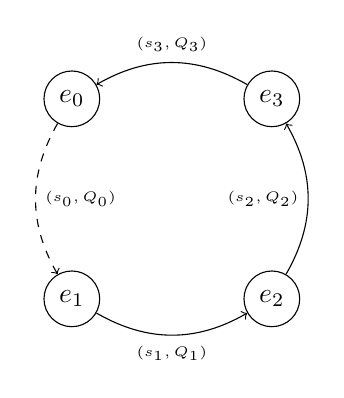
\begin{tikzpicture}[->]%,>=stealth',shorten >=1pt]
    \node[visible on=<8->,draw, circle] (e0) at (-0.5in, 0.5in)     {$\textcolor{black!100}{e_0}$};
    \node[visible on=<2->,draw, circle] (e1) at (-0.5in, -0.5in)   {$\textcolor{black!100}{e_1}$};
    \node[visible on=<4->,draw, circle] (e2) at (0.5in, -0.5in)  {$\textcolor{black!100}{e_2}$};
    \node[visible on=<6->,draw, circle] (e3) at (0.5in, 0.5in)  {$\textcolor{black!100}{e_3}$};

    \path
    (e0) edge[visible on=<9->,bend right, dashed] node[right] {\tiny{\textcolor{black!100}{$(s_0, Q_0)$}}} (e1)
    (e1) edge[visible on=<3->,bend right] node[below = 0.5pt] {\tiny{\textcolor{black!100}{$(s_1, Q_1)$}}} (e2)
    (e2) edge[visible on=<5->,bend right] node[left] {\tiny{\textcolor{black!100}{$(s_2, Q_2)$}}} (e3)
    (e3) edge[visible on=<7->,bend right] node[above = 0.5pt] {\tiny{\textcolor{black!100}{$(s_3, Q_3)$}}} (e0);
    \end{tikzpicture}
    \only<2->{\caption{AOS ring signature (1-of-4)}{}}
    \only<2->{\source{\cite{Borromean}}}
    \end{figure}
	\end{column}
    \end{columns}}
    %\end{frame}
    
    %\begin{frame}{AOS ring signature}
        {\only<11->{\begin{columns}
        \begin{column}{0.635\linewidth}
				\onslide<11-19> {AOS\_VERIFY($m$, $\sigma$, $Q_i$: $0 \leq i \leq r-1)$:
				\begin{enumerate}
					\item<11 -> for $i \gets 0, \dots, r-1$
					\begin{enumerate}
					    \item<11-> $K_i \gets s_iG - e_iQ_i$;
					    \item<12,14,16,18-> $e_{i+1\%r} \gets hash(K_i||m||i+1\%r)$;
					\end{enumerate}
					\item<19 -> \textbf{if} $e_0 = 0$ or $e_0 \geq n$: \\ \textbf{\ \ \ return} False;\\
					\item<19 -> \textbf{if} $e_0 = \sigma[0]$:
					\\ \textbf{\ \ \ return} True;\\
				\end{enumerate}}
			\end{column}
	\begin{column}{0.365\linewidth}
	\begin{figure}
    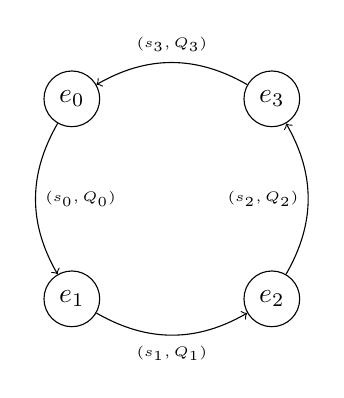
\begin{tikzpicture}[->]%,>=stealth',shorten >=1pt]
    \node[visible on=<18->,draw, circle] (e0) at (-0.5in, 0.5in)     {$\textcolor{black!100}{e_0}$};
    \node[visible on=<12->,draw, circle] (e1) at (-0.5in, -0.5in)   {$\textcolor{black!100}{e_1}$};
    \node[visible on=<14->,draw, circle] (e2) at (0.5in, -0.5in)  {$\textcolor{black!100}{e_2}$};
    \node[visible on=<16->,draw, circle] (e3) at (0.5in, 0.5in)  {$\textcolor{black!100}{e_3}$};

    \path
    (e0) edge[visible on=<11->,bend right] node[right] {\tiny{\textcolor{black!100}{$(s_0, Q_0)$}}} (e1)
    (e1) edge[visible on=<13->,bend right] node[below = 0.5pt] {\tiny{\textcolor{black!100}{$(s_1, Q_1)$}}} (e2)
    (e2) edge[visible on=<15->,bend right] node[left] {\tiny{\textcolor{black!100}{$(s_2, Q_2)$}}} (e3)
    (e3) edge[visible on=<17->,bend right] node[above = 0.5pt] {\tiny{\textcolor{black!100}{$(s_3, Q_3)$}}} (e0);
    \end{tikzpicture}
    \only<11->{\caption{AOS ring signature verification (1-of-4)}}
    \only<11->{\source{\cite{Borromean}}}
    \end{figure}
	\end{column}
    \end{columns}}}
    \end{frame}
    
    \begin{frame}{ECDH Key Exchange protocol}
    \begin{itemize}
        \item Key agreement scheme based on elliptic curve cryptography.
        \item Establish a shared secret between two parties over an insecure (yet authenticated) channel.
    \end{itemize}
    \begin{center}
        \begin{figure}
            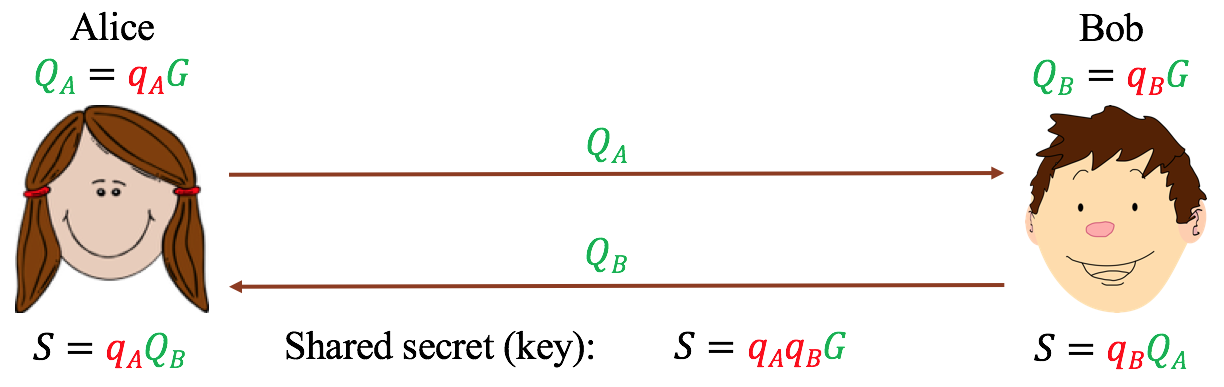
\includegraphics[scale = 0.5]{Images/ECDH.png}
            \captionof{figure}{ECDH key exchange}
        \end{figure}
    \end{center}
    \begin{itemize}
        \item Channel authentication required to prevent \textit{man-in-the-middle} attacks.
    \end{itemize}
    \end{frame}
    
    \begin{frame}{Sender-receiver interaction}
        \begin{itemize}
            \item Encryption even prevents the receiver to know amount and blinding factor associated to each output.
        \end{itemize}
        Transmission of:
        \begin{itemize}
            \item amounts;
            \item blinding factors;
            \item user-selected data.
        \end{itemize}\\ \ \\
        \centering$\Rightarrow$ The transfer can happen non-interactively by running an instance of ECDH and exploiting the shared key to deduce the quantities involved.
    \end{frame}
    
\backupend
\end{document}
  